\documentclass[10pt,twocolumn]{article}
\usepackage[utf8]{inputenc}
\usepackage[T1]{fontenc}
\usepackage{graphicx,booktabs,amsmath,hyperref,geometry}
\geometry{margin=0.75in}
\usepackage[numbers,sort&compress]{natbib}
\title{From Benchmark to Browser: Reproducible Evaluation and CPU-Only Improvement of an On-Device Car-Damage Detector on CarDD}
\author{[Author names --- to be completed]\\ \small Çekicin AI Lab (independent research prototype for roadside-assistance damage pre-assessment)}
\date{Working draft v0.1 --- 19 October 2026 --- not peer reviewed}
\begin{document}
\maketitle
\begin{abstract}
Published car-damage detectors are rarely evaluated in the form in which they are deployed. We benchmark the detector of a browser-based damage pre-assessment tool --- a YOLO11m model quantised to int8 ONNX and executed client-side --- on the official CarDD test split (374 images) with the COCO box protocol used by the CarDD authors. The deployed model reaches 59.9 box AP / 75.7 AP50, below the AP50 of 89.9 claimed on its public model card, and statistically on par with the strongest model of the CarDD paper (DCN+ R101: 60.6 / 78.8). Horizontal-flip test-time augmentation fused with Weighted Boxes Fusion raises this to 62.23 AP / 77.96 AP50 and improves small-object AP from 24.9 to 31.61, with a bit-exact JavaScript port. We then ask how far the frozen detector can be improved with CPU-only training on CarDD. We find that the detector has memorised the training split (79.4 AP on train vs. 64.8 on val), which makes training-split predictions unusable for stacking; a gradient-boosted rescorer fitted on val with grouped cross-validation adds only 0.24 AP on test (paired 95\% CI +0.03 to +0.42). Slicing-aided inference on 2$\times$2 tiles changes test AP to 62.17 (careful mode). Alongside, we review 100 car-damage papers (2019--2026) and distil 100 actionable practices. All predictions, scripts, models and logs are released.
\par\smallskip\noindent\textbf{Keywords:} car damage detection; CarDD; on-device inference; test-time augmentation; weighted boxes fusion; learned rescoring; reproducibility
\end{abstract}
\section{Introduction}
Roadside-assistance operators receive photos of damaged cars from drivers who need to know quickly whether the car can be driven, whether a tow truck is required, and what kind of damage is visible. A detector that runs in the phone browser avoids uploading photos, works on weak networks and costs nothing per request; but it must be small, quantised and fast, and its accuracy must be known under exactly these conditions.

The literature reports many numbers for car-damage detection, but they are hard to compare: in the 100 papers we reviewed, 27 use private insurer data, only 7 use the public CarDD benchmark ~\cite{cardd}, and only 24 state a quantitative result in the abstract. Model cards on public hubs add further claims that are seldom independently checked.

\textbf{Contributions.} (i) We evaluate a deployed, browser-identical int8 detector (a public checkpoint we did not retrain) on the official CarDD test split with the exact COCO protocol ~\cite{coco} of the CarDD paper, and show that a public model-card claim does not reproduce. (ii) We quantify flip test-time augmentation with Weighted Boxes Fusion (WBF) ~\cite{wbf} and ship it with a verified JavaScript port. (iii) We study CPU-only improvements that use the CarDD training data without retraining the network --- a learned rescoring stage and slicing-aided inference --- under a strict protocol (fit on val, select by grouped cross-validation, test once), and report a largely negative result together with its cause: the detector has memorised CarDD train. (iv) We release a 100-paper structured review with 100 derived practices, and all artefacts (detections, scripts, models, experiment logs).

\begin{figure*}[t]\centering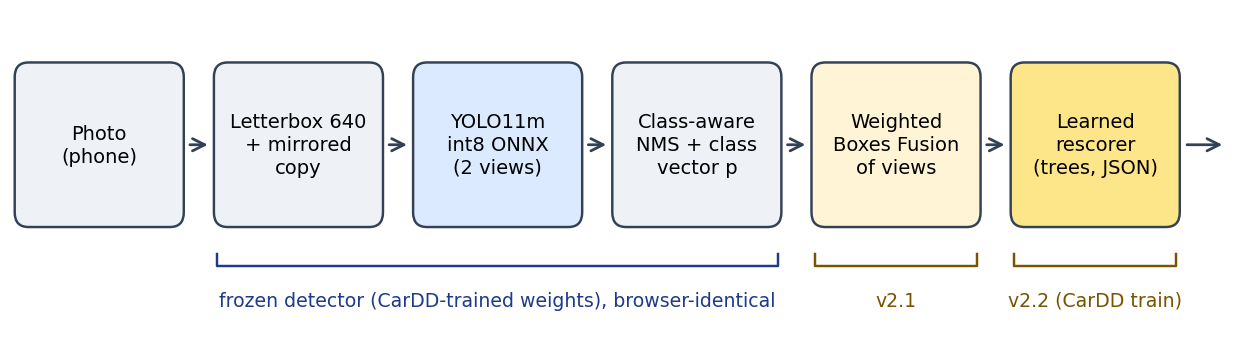
\includegraphics[width=\linewidth]{fig/pipeline.png}\caption{Inference pipeline. Everything runs client-side in the browser; the detector weights are frozen. v2.1 adds the mirrored view and WBF; v2.2 candidates (learned rescorer, tiles) are evaluated in Sec. 5.}\end{figure*}
\section{Related work}
\textbf{Datasets.} CarDD ~\cite{cardd} provides 4,000 images with 9,163 instances of six damage classes (dent, scratch, crack, glass shatter, lamp broken, tire flat) and an official 2,816/810/374 split. Multi-view datasets such as CDDM with the MVA-CDD method ~\cite{mvacdd} fuse close-up and distant views; Small Dents ~\cite{smalldents} targets subtle dents. Our review shows a fast-growing field (28 papers in 2025 and 24 in 2026 among the 100 selected) dominated by private data.

\textbf{Detectors.} The CarDD authors benchmark Mask R-CNN ~\cite{maskrcnn}, HTC and deformable convolutions (DCN) ~\cite{dcn}, and propose DCN+ with multi-scale training and focal loss. Recent work reports YOLOv11 and RT-DETR on CarDD ~\cite{yolov11rtdetr}, enhanced YOLO variants with a damage-severity index ~\cite{enhyolo}, heterogeneous-convolution YOLO ~\cite{hlyolo}, diffusion-based detectors ~\cite{diffdet,cdiffdet} and real-time detection transformers such as RF-DETR ~\cite{rfdetr}. Vision--language models are evaluated for insurance tasks ~\cite{insmm}, grounded with segmentation to reduce hallucination ~\cite{groundvlm}, or used for phrase grounding of damage ~\cite{groundingcardd}.

\textbf{Post-processing.} WBF ~\cite{wbf} averages coordinates of overlapping boxes from several models or augmentations. Localisation-quality estimation (IoU-Net ~\cite{iounet}, VarifocalNet ~\cite{vfnet}) and learned NMS ~\cite{learnnms} show that the detector confidence is not always the best ranking signal; our rescorer is a light-weight, post-hoc instance of this idea using gradient-boosted trees ~\cite{gbm,lightgbm}.

\section{System and evaluation protocol}
\textbf{Detector.} The deployed detector is a public YOLO11m ~\cite{yolo11} checkpoint (\texttt{shanexf/car-damage-yolo11m-ft}) that its author fine-tuned for 30 epochs on CarDD images plus photos of intact cars with empty labels, to suppress false alarms on undamaged glass, lamps and reflections. We did not retrain it: we exported it to ONNX and dynamically quantised it to int8 (20.6 MB). Inputs are letterboxed to 640$\times$640; the network output holds 8,400 anchors with 4 box values and 6 class scores. The browser applies arg-max classification, class-aware NMS at IoU 0.45 and keeps the top boxes.

\textbf{Browser parity.} We evaluate with a Python port of the browser pipeline. A vectorised re-implementation reproduces all boxes, classes and scores of the original port (100\% of compared boxes, $\Delta$score < 10⁻⁴), and the JavaScript WBF matches the Python WBF to 10⁻¹⁶ on saved detections.

\textbf{Protocol.} Following the CarDD paper we report COCO box AP (IoU 0.50:0.95), AP50, AP75 and AP for small (< 32$^2$ px), medium and large objects with pycocotools, at confidence $\ge$ 0.001 and at most 100 detections per image. Mean CPU latency is 496 ms per image and view (2 cores, onnxruntime).

\section{Methods}
\subsection{Flip test-time augmentation with WBF}
The photo and its horizontal mirror are processed independently; mirrored boxes are mapped back and both lists are fused with WBF at IoU 0.55. The fused box is the confidence-weighted mean of its members and the fused score is

\begin{equation}\tilde{s} = \frac{1}{n}\sum_{k=1}^{n} s_k \cdot \frac{\min(n, L)}{L}\end{equation}
where $n$ is the number of member boxes and $L = 2$ the number of views, so boxes seen in only one view are down-weighted.

\subsection{Learned rescoring trained on CarDD}
For every candidate box we compute 39 cheap features (44 in careful mode): detector score and class, the full 6-class probability vector of the source anchor (its maximum, margin and entropy), geometry (log-area, aspect, position, distance to the border), image context (rank within class, ratio to the best box of the class, number of overlapping same-class boxes, containment in a higher-scoring box, maximum overlapping score per class, image-level maximum per class) and --- in careful mode --- the per-view scores, their difference, the number of fused members and the IoU between the two views. Multi-label candidates are added for non-arg-max classes with probability $\ge$ 0.01.

The target is the localisation quality $q$ = maximum IoU with a ground-truth box of the same class (0 for false positives). A histogram gradient-boosting regressor predicts $\hat{q}$, and the final score is a geometric blend

\begin{equation}s^{*} = \hat{q}^{\,\alpha}\, s^{\,1-\alpha}\end{equation}
The trees are exported to JSON and evaluated in the browser (identical predictions to scikit-learn on all test candidates when compared in float64).

\subsection{Slicing-aided inference}
To address the weak small-object AP, the photo is cut into 2$\times$2 tiles with 25\% overlap; each tile is letterboxed to 640 px, so objects appear about 1.7$\times$ larger. Tile boxes touching an inner tile border are discarded, duplicates across tiles are removed by NMS, and tile boxes are fused with the full-image detections either by WBF, by NMS, or by a complement rule that only adds tile boxes not explained by a full-image box; the tile-score weight and a maximum box area are tuned on val.

\section{Experiments}
\subsection{Deployed model vs. published results}
\begin{table*}[t]\centering\small\caption{Box detection on the official CarDD test split (374 images). Paper rows are taken from Table IV of the CarDD paper ~\cite{cardd} unless marked; † = split may differ from the official one.}\resizebox{\linewidth}{!}{\begin{tabular}{lccccc}\toprule
Method & Source & AP & AP50 & AP75 & APs \\\midrule
Mask R-CNN R50 & CarDD ~\cite{cardd} & 49.2 & 66.3 & 52.6 & -- \\
Mask R-CNN R101 & CarDD ~\cite{cardd} & 51.1 & 67.7 & -- & -- \\
DCN R101 & CarDD ~\cite{cardd} & 54.3 & 69.8 & -- & -- \\
DCN+ R50 & CarDD ~\cite{cardd} & 58.8 & 77.4 & 63.1 & -- \\
DCN+ R101 (best) & CarDD ~\cite{cardd} & 60.6 & 78.8 & 64.8 & 37.1 \\
Enhanced YOLOv9 † & ~\cite{enhyolo} & 58.0 & 73.0 & -- & -- \\
YOLOv11m † & ~\cite{yolov11rtdetr} & 63.3 & -- & -- & -- \\
YOLO11m int8, deployed (fast) & ours & 59.9 (95\% CI 56.8--63.2) & 75.7 & 62.0 & 24.9 \\
\textbf{+ flip TTA + WBF (careful, v2.1)} & \textbf{ours} & \textbf{62.23 (95\% CI 59.5--65.4)} & \textbf{77.96} & \textbf{64.40} & \textbf{31.61} \\
\bottomrule\end{tabular}}\end{table*}
The deployed model matches the best CarDD-paper model in AP and is 3.1 points lower in AP50. The careful mode has a higher point estimate than DCN+ R101 (62.23 vs. 60.6 AP) and is within one point in AP50, but the image-bootstrap 95\% interval (95\% CI 59.5--65.4) contains 60.6: the two are \textbf{on par}, not distinguishable on 374 test images. The gain of careful over fast mode, in contrast, is clear: +2.33 AP (95\% CI +1.48 to +3.15; positive in 100\% of 150 resamples). The AP50 of 89.9 stated on the public model card of the base weights is \textbf{not reproduced} (75.7). The card states that training and evaluation used the author's own fixed 80/10/10 hash split of the labelled CarDD images rather than the official split; together with the memorisation analysis below (AP50 92.9 on official-train images) this suggests that the card's test images overlap the official training images, so the claim is not comparable with published CarDD results. Raising the on-device confidence threshold costs accuracy (AP 57.8 at 0.05, 56.4 at 0.25).

\begin{table}[t]\centering\small\caption{Per-class box AP / AP50 on CarDD test. The CarDD-paper column is \emph{mask} AP (Table II of ~\cite{cardd}) and is shown for orientation only.}\resizebox{\linewidth}{!}{\begin{tabular}{lccccc}\toprule
Class & fast AP & fast AP50 & careful AP & careful AP50 & DCN+ R101 mask AP \\\midrule
dent & 33.0 & 58.2 & 37.7 & 64.1 & 40.5 \\
scratch & 38.1 & 66.5 & 42.1 & 69.9 & 34.3 \\
crack & 31.6 & 52.1 & 32.3 & 53.8 & 16.6 \\
glass shatter & 93.2 & 97.2 & 93.4 & 97.3 & 89.6 \\
lamp broken & 76.9 & 88.3 & 80.9 & 90.8 & 70.8 \\
tire flat & 86.8 & 91.4 & 87.0 & 91.9 & 90.0 \\
\bottomrule\end{tabular}}\end{table}
\subsection{Memorisation of the training split}
Before fitting anything on CarDD we ran the deployed detector on all three splits. AP is 79.4 on the first 250 training images, 64.8 on val and 59.9 on test (AP50 92.9 / 79.2 / 75.7). The detector has memorised the training images, and val is also optimistic (it was probably used for checkpoint selection). Predictions on train are therefore not representative of deployment, and any second stage fitted on them would learn from over-confident scores. We fit all post-hoc components on \textbf{val} and select hyper-parameters by 5-fold cross-validation grouped by image; test is evaluated once.

\subsection{Learned rescoring}
\begin{table}[t]\centering\small\caption{Learned rescoring on CarDD test. Fitted on val (18163 candidate boxes in careful mode); hyper-parameters (4 tree configurations $\times$ 5 iteration counts $\times$ 4 blends) chosen by out-of-fold AP.}\resizebox{\linewidth}{!}{\begin{tabular}{lcccc}\toprule
Mode & CV AP before $\rightarrow$ after & test AP before $\rightarrow$ after & test AP50 & test APs \\\midrule
fast & 64.75 $\rightarrow$ 64.90 & 59.93 $\rightarrow$ 60.08 & 75.62 $\rightarrow$ 75.90 & 25.15 $\rightarrow$ 25.24 \\
careful & 66.56 $\rightarrow$ 66.57 & 62.23 $\rightarrow$ 62.47 & 77.96 $\rightarrow$ 78.09 & 31.61 $\rightarrow$ 31.72 \\
\bottomrule\end{tabular}}\end{table}
Rescoring yields small gains: +0.23 AP (95\% CI +0.03 to +0.42; positive in 99\% of 150 resamples) in careful mode and +0.16 AP (95\% CI +0.00 to +0.33; positive in 97\% of 150 resamples) in fast mode (paired image bootstrap ~\cite{efron}). Permutation importance explains why: in fast mode the detector score alone accounts for most of the predictive power (0.87 vs. $\le$ 0.05 for any other feature), i.e. the single-view confidence is already close to the best ranking these features allow. In careful mode the per-view scores and the class probability carry complementary signal, which is where the (small) gain comes from. Multi-label candidates alone do not change AP (careful 62.26 vs. 62.23).

\subsection{Slicing-aided inference}
\begin{table}[t]\centering\small\caption{Tiled inference (2$\times$2, 25\% overlap) fused with the full-image detections; fusion rule, maximum tile-box area and tile-score weight chosen on val.}\resizebox{\linewidth}{!}{\begin{tabular}{lcccc}\toprule
Setting & val AP & test AP & test AP50 & test APs \\\midrule
Fast (no tiles) & 64.75 & 59.93 & 75.62 & 25.15 \\
Fast + tiles (nms, area $\le$ 0.1, w = 0.3) & 64.95 & 59.92 & 75.65 & 26.82 \\
Careful (no tiles) & 66.56 & 62.23 & 77.96 & 31.61 \\
Careful + tiles (add, area $\le$ 0.01, w = 0.3) & 66.48 & 62.17 & 77.83 & 31.27 \\
\bottomrule\end{tabular}}\end{table}
On val, the best of 48 tile configurations improved fast mode only slightly (+0.20 AP) and none improved careful mode (best -0.08). On test, tiling changes AP by -0.01 (fast) and -0.06 (careful); paired bootstrap for careful mode: -0.07 AP (95\% CI -0.14 to +0.05; positive in 13\% of 150 resamples). Small-object AP rises in fast mode (+1.67) but not in careful mode (-0.34), where the mirrored view already recovers many small objects. CarDD photos are mostly close-ups in which damage is already large relative to the 640-px input, and extra tile boxes add false positives and truncated boxes on larger damage; tiling also multiplies compute by five. We therefore do not adopt it; it may still help on wide shots of whole cars, which CarDD does not cover.

\section{Discussion and limitations}
\begin{itemize}\item \textbf{Licence.} CarDD is released for non-commercial research. A commercial service needs either a licence or a model retrained on consented operator photos.
\item \textbf{Leakage risk.} The base weights were trained by a third party on a re-split of CarDD; we cannot verify that no official test image was used. The ordering train ≫ val > test suggests limited overlap with the official test split, but a clean comparison requires retraining from generic (COCO) weights on the official training split only --- the setting of our released GPU notebook.
\item \textbf{Box vs. mask.} CarDD-paper per-class figures are mask AP; our model predicts boxes only.
\item \textbf{Single benchmark.} CarDD images are mostly close-ups from the web; on our own 1,000-photo image-level test (whole cars and close-ups, including intact cars) the same system reaches F1 0.626 with a 14.8\% false-alarm rate on intact whole cars, which is the more relevant figure for operations.
\item \textbf{What CPU-only training can and cannot do.} Without retraining the network, post-hoc stages recover at most a few tenths of an AP point. Larger gains require GPU training --- e.g. RF-DETR ~\cite{rfdetr} or multi-scale training as in DCN+ --- for which we release a ready notebook.
\end{itemize}
\section{Review of 100 papers and 100 derived practices}
We queried OpenAlex ~\cite{openalex} and arXiv for car-damage detection, assessment and insurance-claim papers, obtaining more than 2,400 candidates, filtered off-topic work with a negative-term list and title penalties, and ranked by topical relevance, citations and recency. For the 100 selected papers we extracted models, datasets, tasks, techniques and reported metrics from abstracts (the 12 seed papers were checked by hand). The most frequent model families are Transfer learning (25), YOLOv8 (15), Mask R-CNN (15), ResNet (11), VGG (8), YOLO (7); tasks are detection (87), severity (46), classification (44) and segmentation (22); the most frequent technique themes are lightweight / mobile deployment (42), severity / cost estimation (34), transfer learning / pre-training (26), instance segmentation masks (20). From these we derived 100 practices in eight groups (data and evaluation, detection models, training, inference and fusion, decision layer, severity and cost, VLM/LLM use, deployment and operations); 46 were already implemented, 8 were added in v2.1, 27 are planned on CPU and 19 require GPU training.

\section{Conclusion}
A browser-deployed int8 YOLO11m is on par with the best model in the CarDD paper when evaluated under the same protocol, and flip-TTA with WBF adds a significant +2.3 AP (62.23 AP). Training post-hoc stages on CarDD without a GPU yields only marginal further gains, and we identify memorisation of the training split as a pitfall that silently invalidates stacking on training predictions. The next step is GPU retraining on licence-clean data and an evaluation on operator photos.

\section*{Reproducibility}
Detections, scripts and results: Hugging Face datasets \texttt{sosa123454321/cekicin-training-artifacts} (folders v2\_1, v2\_2) and \texttt{sosa123454321/cekicin-ai-papers} (car\_damage\_100). Experiment tracking, models and artefacts: Weights \& Biases project \texttt{elasa2next-sosa-/cekicin-hasar-ai}. Live demo: sosa123454321-cekicin-site.static.hf.space/ai-lab/model-test.html.

\bibliographystyle{unsrtnat}
\bibliography{refs}
\end{document}